\runningheader{Oppgave i)}{}{Side \thepage\ av \numpages}
% ********************************************************
% oppgave i) 
% ******************************************************** 
\item
{\bf FIR-filter}
\label{oppg:i}

I Lego-prosjektet skal du jobbe med 
  FIR-filter (midlingsfilter) gitt som 
\begin{equation}
  \label{eq:MA2}
  y_{k} = \frac{1}{M}\sum_{n=0}^{M-1} x_{k-n}
\end{equation}
hvor $M$ er antall målinger av $x$ som skal være med i midlingen.
I denne oppgaven skal du først implementere kode for filteret i
ligning~\eqref{eq:MA2} og deretter skal du lage en egen
funksjon for FIR-filteret i skallfilen \fbox{\tt FIR\_filter.m}. 

Ta utgangspunkt i skallfilen
hvor du ser at den diskret tidsvektoren
\fbox{\tt t} er basert på en antatt samplingsfrekvens på
  \begin{equation}
    \label{eq:15}
      f_{s} = 10~\text{Hz}
  \end{equation}
  som gir et tidsskritt på
  \begin{equation}
    \label{eq:14}
T_{s} = \frac{1}{f_{s}} = 0.1~\text{sekund}     
  \end{equation}
Med en slutt-tid på 10 sekund  betyr det at vi har 100 målinger
tilgjengelig, og målesignalet \fbox{\tt x} er som du ser bare støy. 
Gjør følgende oppgaver:
\begin{itemize}
\item  Implementer kode for
  FIR-filteret i ligning~\eqref{eq:MA2} i {\it for}-løkken. Vær nøye med
  indeksene.
  
  Der hvor det står {\color{darkgreen}\fbox{\tt \% juster på M her}} så gjelder dette
  for situasjonen hvor $k{<}M$ hvor det ikke er nok
  målinger til å bruke {\tt M = 10}. En måte å løse det på er å utsette
  filtreringen til $k{>}M$, men en bedre løsning er justere på $M$
  slik at filtreringen kan starte med en gang.
  Hint: Hva skulle du ønske at
  $M$ var i starten av filtreringen, og så lenge $k{<}M$?

  Vær
  klar over at siden du gjør justeringer på $M$ inne i {\it for}-løkka
  når $k < M$, så må koden \fbox{\tt M = 10;} stå inne i den samme
  løkka. Setter du koden {\tt M = 10;} foran {\it for}-løkka så vil
  ikke verdien av $M$ bli resatt for hver runde i løkka. Test det
  gjerne ut.

\newpage
  Ferdigstill og kjør koden og vis at du får  resultatet vist i figur~\ref{fig:3i}.
    \begin{figure}[H]
      \centering
      \hspace*{0mm}\scalebox{0.45}{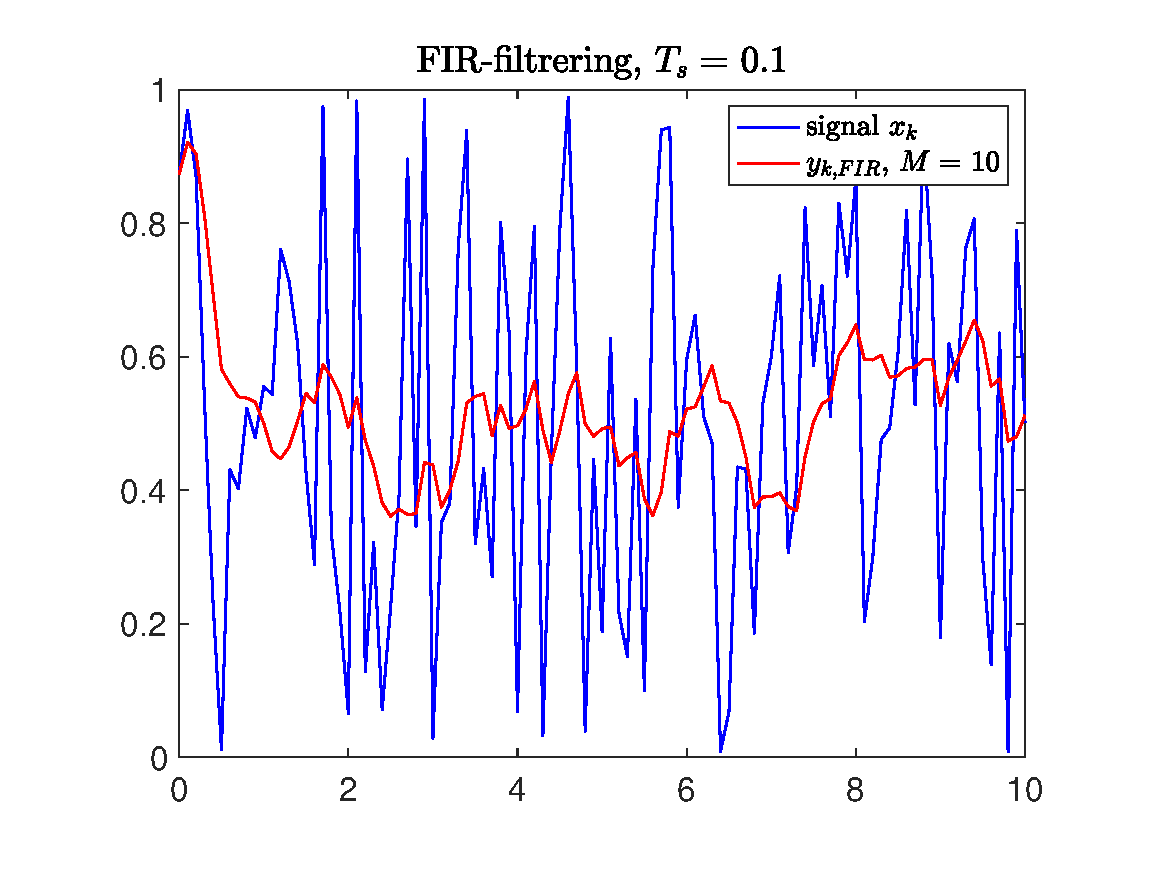
\includegraphics{3i.pdf}}
      \caption{Respons i FIR-filter med $M{=}10$. }
      \label{fig:3i}
    \end{figure}
    
    
\item Innholdet  i skallfilen \fbox{\tt FIR\_filter.m} er
  vist under, og som du ser benyttes beskrivende matematiske
  variabelnavn i  funksjonen. 

\begin{lstlisting}[caption={Skall for funksjonen for FIR-filtrering.},
 language= Matlab,   label=kode:FIR_funk,
numbers=none] 
function FilteredValue = FIR_filter(Measurement, NoOfMeas)

% juster på NoOfMeas her
% fyll inn filterkode

end
\end{lstlisting}
Ferdigstill koden i denne funksjonen. 
  Legg merke til at vi flytter 
  koden som justerer på $M$ inn i funksjonen. På den måten  blir mer
  funksjonen mer funskjonell i bruk, og $M$ kan spesifiseres 
  før  {\it for}-løkken i hovedfilen.
  

\item Vis at du får samme resultat som i figur~\ref{fig:3i} ved å
  endre {\it for}-løkken i skallfilen til
  
\begin{lstlisting}[caption={Syntaks for å kalle funksjonen {\tt FIR\_filter}.},
 language= Matlab,   label=kode:FIR_funk_kall,
numbers=none] 
M = 10;
for k = ..
    y_FIR(k) = FIR_filter(.., ..)
end
\end{lstlisting}

% Som du ser så sendes det inn målinger frem til og med
% indeks $k$, {\tt x(1:k)}. For å forstå hvorfor
% du må gjøre det på denne måten, prøv å send inn 
% alle målingene i {\tt x}  og se hva som  skjer, altså at kallet ser
% slik ut
% \fbox{\tt y\_FIR(k) = FIR\_filter(x, M)}. 

\subsubsection*{Effekten av $M$}
  
\item   For å teste betydningen av verdien på $M$ så
  er det i skallfilen {\tt oving3\_skallfil.m} laget til en egen
  seksjon som du kan kjøre direkte når du har laget ferdig funksjonen
  {\tt FIR\_filter}.  
  Vis at du får resultatet vist i  figur~\ref{fig:3i2}. 

    \begin{figure}[H]
      \centering
      \hspace*{0mm}\scalebox{0.5}{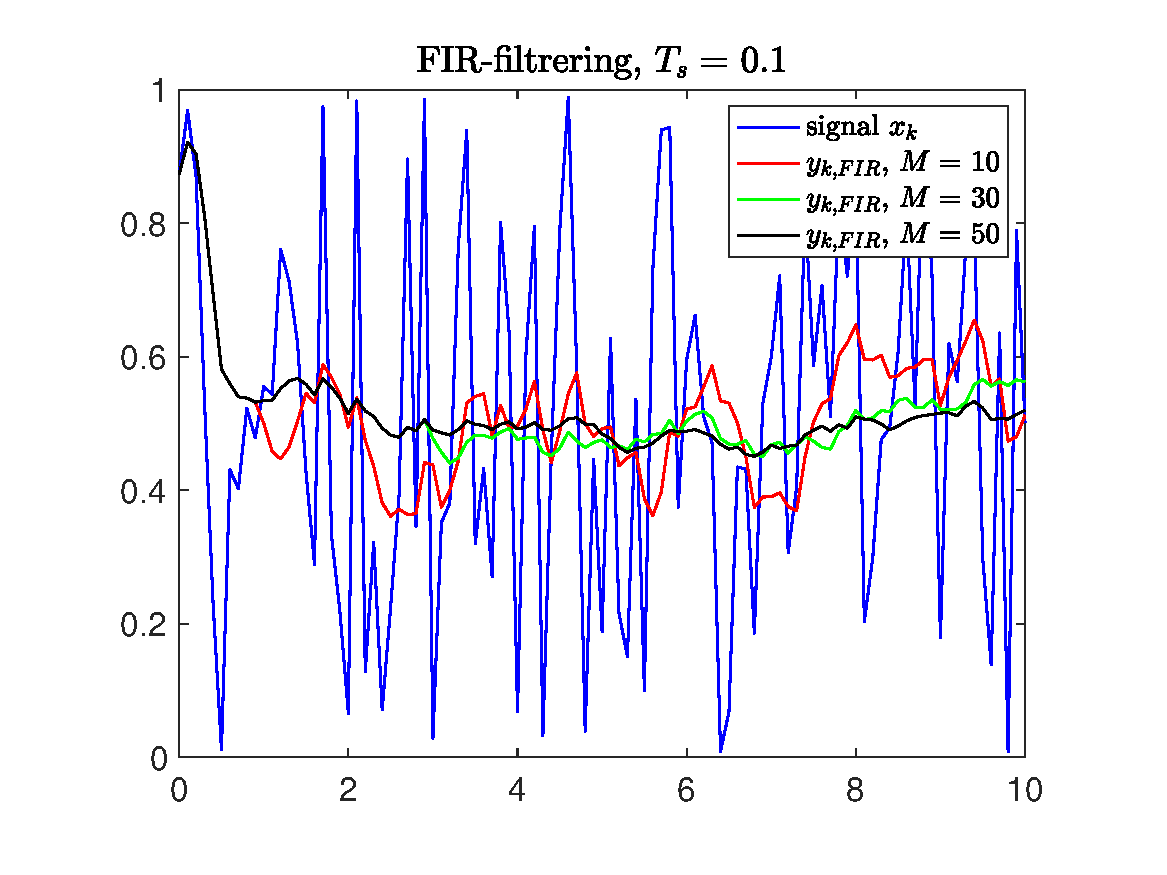
\includegraphics{3i2.pdf}}
      \caption{Respons i FIR-filter med $M{=}[10, 30, 50]$. }
      \label{fig:3i2}
    \end{figure}

    \item Hva er grunnen til at alle de tre filtrerte kurvene ligger over hverandre frem til
      ca 1 sekund? Samme fenomen ser du gjelder for 
      to av kurvene mellom 1 og 3 sekund. 

    \item  Er filtreringen som oppnås fornuftig i forhold til stigende
      tall på $M$? Begrunn svaret.

      \item Lek gjerne med andre verdier på $M$. Hva skjer hvis du
        setter \fbox{\tt M = k;} inne i {\it for}-løkken? 
\end{itemize}

